\documentclass[journal]{IEEEtran}
\usepackage[T1]{fontenc}
\usepackage[utf8]{inputenc}
\usepackage{amsmath,amssymb}
\usepackage{graphicx}
\usepackage{booktabs}
\usepackage{caption}
\usepackage{subcaption}
\usepackage[hidelinks]{hyperref}
\renewcommand{\ttdefault}{cmtt}
\urlstyle{same}
\graphicspath{{figures/}}
\newcommand{\relay}{R.E.L.A.Y.}
\newcommand{\pcu}{PCU}

% Supplementary floats are numbered S1, S2, ... and T-S1, so they cannot be confused
% with the figures and tables of the main manuscript.
\renewcommand{\thefigure}{S\arabic{figure}}
\renewcommand{\thetable}{S\arabic{table}}

\title{Supplementary Material\\
A Low-Cost Single-Camera Adaptive Signal Controller for Heterogeneous Urban Traffic}
\author{Niraj~Kafle}

\begin{document}
\maketitle

This supplement holds the unaggregated and per-class results referenced from the main manuscript.
Nothing here is required to follow the argument; it is provided so every reported number can be
inspected at the level it was measured.

\begin{figure}[t]
\centering
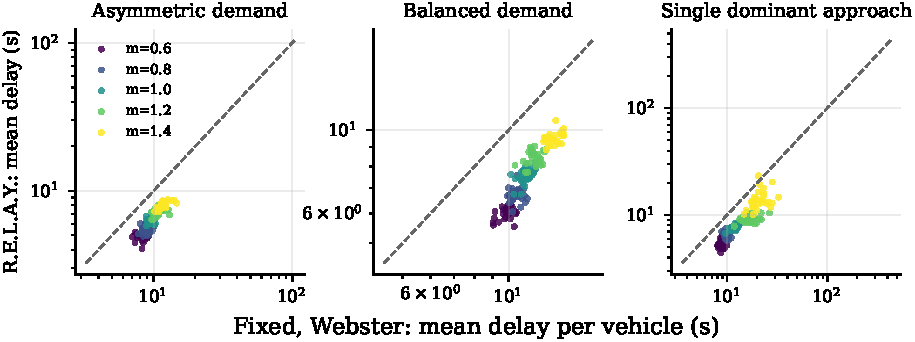
\includegraphics[width=\textwidth]{exp1_paired.pdf}
\caption{Experiment 1, unaggregated. Each point is one seed at one demand level, plotting \relay's
mean delay against the Webster plan's mean delay on the identical arrival stream. Points below the
diagonal favour \relay. Colour encodes the demand multiplier from 0.6 (dark) to 1.4 (light).}
\label{fig:exp1paired}
\end{figure}

\begin{figure}[t]
\centering
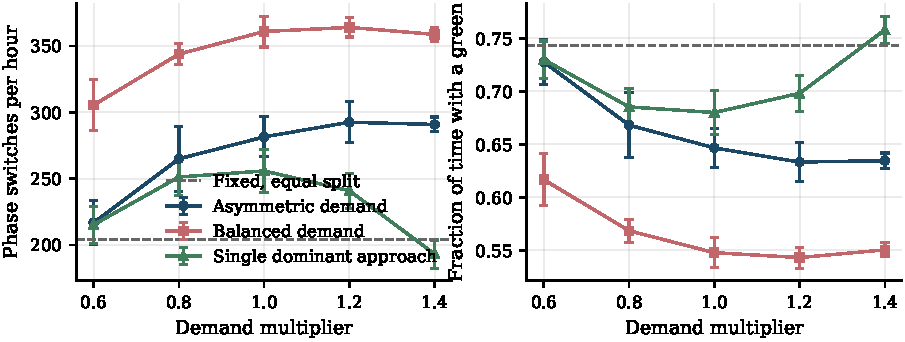
\includegraphics[width=\textwidth]{exp1b_switching.pdf}
\caption{Experiment 1b. Left: phase changes per hour. Right: the fraction of wall time during which
a green is displayed, the complement of which is time spent in yellow and all-red clearance. The
dashed line is the equal-split fixed plan, whose behaviour is independent of demand by construction.}
\label{fig:exp1b}
\end{figure}

\begin{figure}[t]
\centering
\begin{subfigure}{\textwidth}
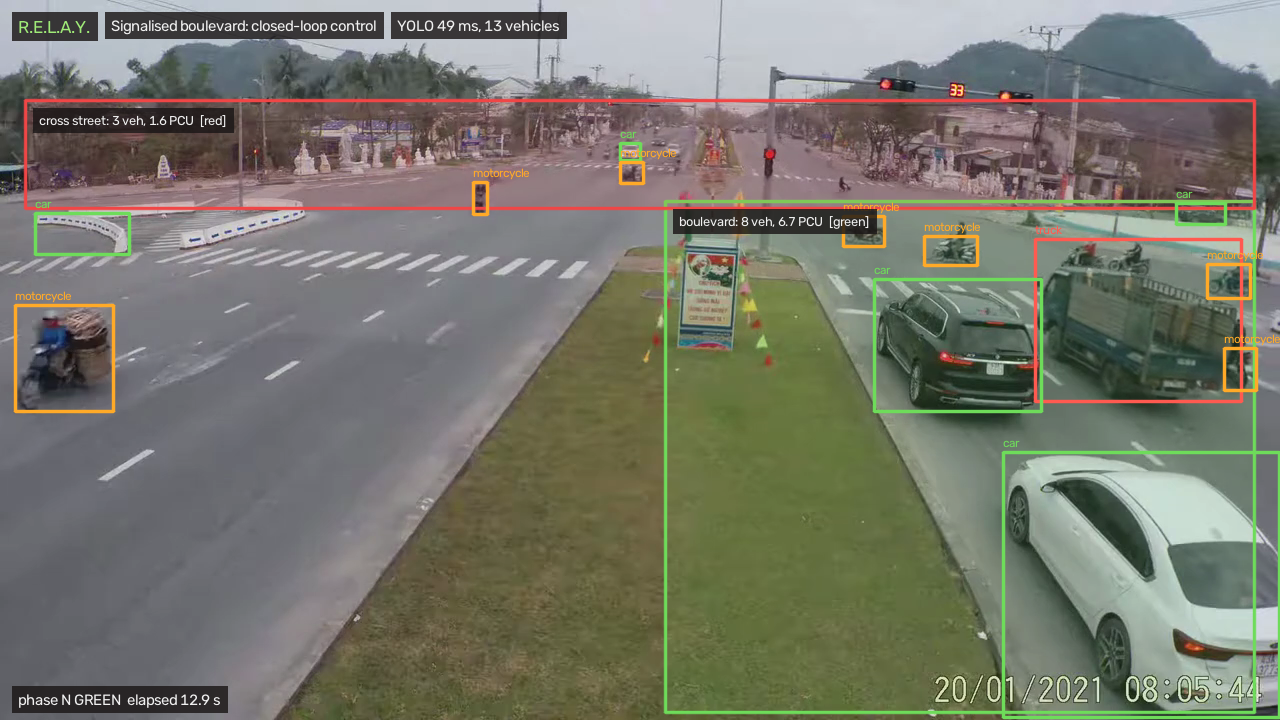
\includegraphics[width=\textwidth]{frame_levanhien_22s.png}
\caption{Signalised boulevard. The controller is running on these counts: the near boulevard approach
holds 8 vehicles and 6.7~\pcu{} and has green, the crossing street holds 3 vehicles and 1.6~\pcu{}
and is red, and the header reports the real inference latency for the frame.}
\end{subfigure}
\vspace{0.5em}
\begin{subfigure}{\textwidth}
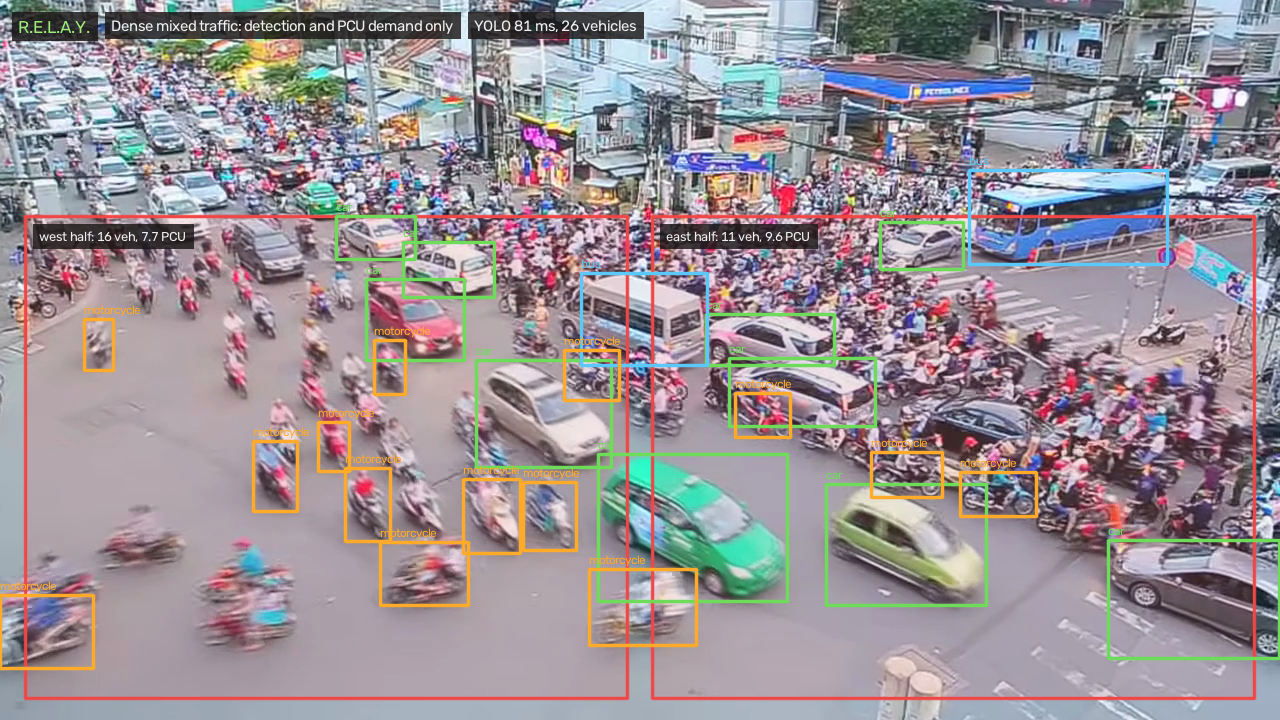
\includegraphics[width=\textwidth]{frame_hcmc_18s.png}
\caption{Dense motorcycle-dominated traffic. The failure mode is visible: 26 vehicles are detected in
a scene containing several hundred, so the reported \pcu{} demand of 7.7 and 9.6 for the two halves
is a severe underestimate. No controller decision is shown, because the junction depicted is not
signal-controlled in the way the two zones imply.}
\end{subfigure}
\caption{Experiment 4. The perception stack on real fixed-camera footage. Both frames are direct
output of the system, with detections, approach polygons and per-approach \pcu{} demand as computed
at run time.}
\label{fig:frames}
\end{figure}

\begin{table}[t]
\centering
\caption{Experiment 4. Detector performance on the system's held-out split: 97 images, 4990 labelled
instances. The checkpoint evaluated is the one shipped with the system, a 2.59-million parameter
model. P and R are precision and recall at the operating point the validator reports.}
\label{tab:detector}
\footnotesize
\setlength{\tabcolsep}{4.5pt}
\begin{tabular}{lccccccccc}
\toprule
& \multicolumn{4}{c}{Overall} & \multicolumn{5}{c}{AP@50 by class} \\
\cmidrule(lr){2-5}\cmidrule(lr){6-10}
Model & mAP@50 & mAP@50-95 & P & R & car & motorcycle & bus & truck & ambulance \\
\midrule
Shipped fine-tune & 0.954 & 0.809 & 0.950 & 0.886 & 0.985 & 0.851 & 0.981 & 0.964 & 0.987 \\
\bottomrule
\end{tabular}
\end{table}

\begin{figure}[t]
\centering
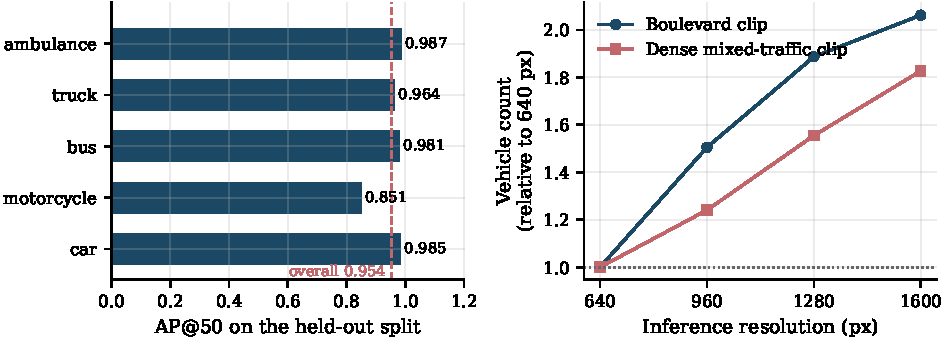
\includegraphics[width=\textwidth]{detector.pdf}
\caption{Experiment 4. Left: per-class average precision at IoU 0.5 on the held-out split, with the
overall mean average precision marked. Right: sampled vehicle count as a function of inference
resolution, normalised to the count at 640~px. Neither curve has flattened by 1600~px, which is
direct evidence that vehicles are still being missed.}
\label{fig:detector}
\end{figure}

\end{document}
